\documentclass[a4paper,11pt]{article}
\usepackage[polish]{babel}
\usepackage{amsmath}
\usepackage[T1]{fontenc}
\usepackage[margin=0.7in]{geometry}
\addtolength{\topmargin}{-.2in}
\usepackage{pythonhighlight}
\usepackage{blindtext}
\usepackage{graphicx}
\usepackage{multicol}
\usepackage{bbding}
\usepackage{caption}
\usepackage{subcaption}
\usepackage{pdfpages}
\usepackage{listings}
\usepackage{url}
\usepackage{float}

\title{Symulator tomografu}
\author{Informatyka w medycynie \\ Michał Miłek 151824 \\ Sebastian Nowak 152065}
\date{\today}

\begin{document}
    \maketitle
    \section{Skład grupy}
    Michał Miłek (151824) \& Sebastian Nowak (152065)

    \section{Model tomogramu}
    W naszym projekcie użyto stożkowego modelu tomogramu.

    \section{Język programowania i biblioteki}
    Nasz projekt został napisany w języku programowania Python,
    wizualizacja została wykonana za pomocą Jupyter Notebook'a.
    Użyte biblioteki to:
    \begin{itemize}
    \item Python Imaging Library (wczytywanie obrazu)
    \item NumPy (niezbędne obliczenia)
    \item skimage (operacje na obrazach)
    \item matplotlib (wizualizacja wyników)
    \item pydicom (zapis i odczyt plików DICOM)
    \end{itemize}

    \section{Opis głównych funkcji programu}
    \subsection{Pozyskiwanie wyników detektorów}
    Do pozyskania wyników detektorów zostały użyte dwie funkcje radon\_transform
    oraz avg brightness (funkcja pomocniczna dla radon\_transform) które zostaną pokazane w oddzielnych skrawkach poniżej.
    \begin{lstlisting}[language=Python, caption=Radon transform, basicstyle=\tiny]
def radon_transform(image, alpha=2, phi_range=90, num_detectors=180, num_iterations=90):
    height, width = image.shape
    radius = int(np.sqrt(height**2 + width**2) / 2)
    x_offset = width // 2
    y_offset = height // 2
    phi_rad = np.radians(phi_range)

    sinogram = np.asarray([[0 for i in range(num_detectors)] for j in range(num_iterations)])

    for i in range(num_iterations):
        curr_alpha = i * np.radians(alpha)
        xe = int(radius * np.cos(curr_alpha)) + x_offset
        ye = int(radius * np.sin(curr_alpha)) + y_offset

        for j in range(num_detectors):
            xd = int(radius * np.cos(curr_alpha + np.pi - (phi_rad / 2) + j * phi_rad/(num_detectors-1))) + x_offset
            yd = int(radius * np.sin(curr_alpha + np.pi - (phi_rad / 2) + j * phi_rad/(num_detectors-1))) + y_offset
            sinogram[i][j] = avg_brightness(line_nd([xe, ye], [xd, yd]), image)
    return sinogram
  \end{lstlisting}

  \begin{lstlisting}[language=Python, caption=Average brightness, basicstyle=\tiny]
def avg_brightness(line, image):
    width, height = image.shape
    sum = 0
    line = list(zip(line[0], line[1]))
    for [x, y] in line:
        if (x < 0 or x >= width) or (y < 0 or y >= height):
            continue
        sum += image[x,y]
    return int(sum / len(line))    
  \end{lstlisting}
  
  \subsection{Uśrednianie wyniku}
  Uśrednianie wyniku jest w funkcji backprojection a funkcja pomocniczna w uśrednianiu (draw\_line) będzie przedstawiona w następnym skrawku kodu.
  \begin{lstlisting}[language=Python, caption=Backprojection, basicstyle=\tiny]
def backprojection(image, sinogram, alpha=2, phi_range=90, num_detectors=180, num_iterations=90):
    height, width = image.shape
    radius = int(np.sqrt(height**2 + width**2) // 2)
    x_offset = width // 2
    y_offset = height // 2
    phi_rad = np.radians(phi_range)

    reconstruction = np.asarray([[0 for i in range(image.shape[0])] for j in range(image.shape[1])])
    pixel_counter = np.asarray([[1 for i in range(image.shape[0])] for j in range(image.shape[1])])

    for i in range(num_iterations):
        curr_alpha = i * np.radians(alpha)
        xe = int(radius * np.cos(curr_alpha)) + x_offset
        ye = int(radius * np.sin(curr_alpha)) + y_offset

        for j in range(num_detectors):
            xd = int(radius * np.cos(curr_alpha + np.pi - (phi_rad / 2) + j * phi_rad/(num_detectors-1))) + x_offset
            yd = int(radius * np.sin(curr_alpha + np.pi - (phi_rad / 2) + j * phi_rad/(num_detectors-1))) + y_offset
            reconstruction = draw_line(line_nd([xe, ye], [xd, yd]), reconstruction, i, j, pixel_counter, sinogram)

    for y, x in np.ndindex(reconstruction.shape):
        reconstruction[x][y] = reconstruction[x][y] / pixel_counter[x][y]
    return reconstruction
  \end{lstlisting}

  \begin{lstlisting}[language=Python, caption=Draw line, basicstyle=\tiny]
def draw_line(line, image, i, j, pixel_counter, sinogram):
    height, width = image.shape
    line = list(zip(line[0], line[1]))
    for [y, x] in line:
        if (x < 0 or x >= height) or (y < 0 or y >= width):
            continue
        image[x][y] += sinogram[i][j]
        pixel_counter[x][y] += 1
    return image
  \end{lstlisting}

  \subsection{Zapis i odczyt plików DICOM}
  W skrawkach poniżej będzie kolejno pokazany zapis a potem odczyt plików DICOM.
  \begin{lstlisting}[language=Python, caption=save DICOM file, basicstyle=\tiny]
def save_as_dicom(file_name, img, patient_data):
    img = convert_image_to_ubyte(img)
    # Populate required values for file meta information
    meta = Dataset()
    meta.MediaStorageSOPClassUID = pydicom._storage_sopclass_uids.CTImageStorage
    meta.MediaStorageSOPInstanceUID = pydicom.uid.generate_uid()
    meta.TransferSyntaxUID = pydicom.uid.ExplicitVRLittleEndian  

    ds = FileDataset(None, {}, preamble=b"\0" * 128)
    ds.file_meta = meta

    ds.is_little_endian = True
    ds.is_implicit_VR = False

    ds.SOPClassUID = pydicom._storage_sopclass_uids.CTImageStorage
    ds.SOPInstanceUID = meta.MediaStorageSOPInstanceUID

    ds.PatientName = patient_data["PatientName"]
    ds.PatientID = patient_data["PatientID"]
    ds.ImageComments = patient_data["ImageComments"]

    ds.Modality = "CT"
    ds.SeriesInstanceUID = pydicom.uid.generate_uid()
    ds.StudyInstanceUID = pydicom.uid.generate_uid()
    ds.FrameOfReferenceUID = pydicom.uid.generate_uid()

    ds.BitsStored = 8
    ds.BitsAllocated = 8
    ds.SamplesPerPixel = 1
    ds.HighBit = 7

    ds.ImagesInAcquisition = 1
    ds.InstanceNumber = 1

    ds.Rows, ds.Columns = img.shape

    ds.ImageType = r"ORIGINAL\PRIMARY\AXIAL"

    ds.PhotometricInterpretation = "MONOCHROME2"
    ds.PixelRepresentation = 0

    pydicom.dataset.validate_file_meta(ds.file_meta, enforce_standard=True)

    ds.PixelData = img.tobytes()

    ds.save_as(file_name, write_like_original=False)
    print("Saved successfully")    
  \end{lstlisting}
  \begin{lstlisting}[language=Python, caption=read DICOM file, basicstyle=\tiny]
def read_from_dicom(path):
    ds = dcmread(path, force=True)

    # Normal mode:
    print()
    print(f"File path........: {path}")
    print(f"SOP Class........: {ds.SOPClassUID} ({ds.SOPClassUID.name})")
    print()

    pat_name = ds.PatientName
    print(f"Patient's Name...: {pat_name.family_comma_given()}")
    print(f"Patient ID.......: {ds.PatientID}")
    print(f"Modality.........: {ds.Modality}")
    print(f"ImageComments....: {ds.ImageComments}")
    print(f"Image size.......: {ds.Rows} x {ds.Columns}")

    # plot the image using matplotlib
    plt.imshow(ds.pixel_array, cmap=plt.cm.gray)
    plt.show()
    
  \end{lstlisting}

  \section{Przykłady działania}
  \subsection{Przykład 1.}
  
  \begin{figure}[H]
    \centering
    
\includegraphics[scale=0.5]{Kropka.jpg}
    \caption{Przykładowy obraz wejściowy "Kropka.jpg"}
  \end{figure}
  
    \begin{figure}[H]
    \centering
    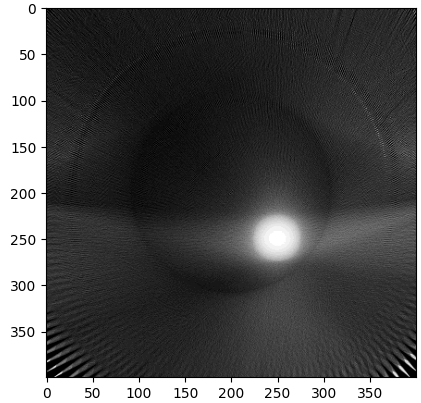
\includegraphics[scale=0.4]{Kropka_reconstructed.png}
    \caption{Zrekonstruowany obraz "Kropka.jpg"}
  \end{figure}

  \subsection{Przykład 2.}
  
  \begin{figure}[H]
    \centering
    
\includegraphics[scale=0.32]{Kwadraty2.jpg}
    \caption{Przykładowy obraz wejściowy "Kwadraty2.jpg"}
  \end{figure}
  
    \begin{figure}[H]
    \centering
    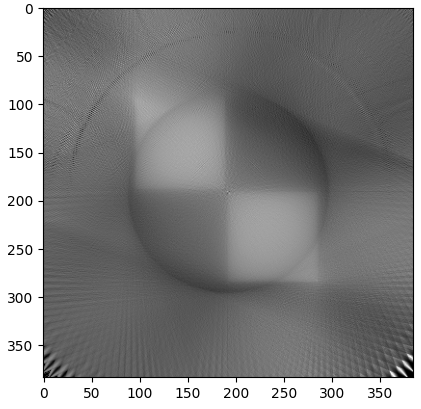
\includegraphics[scale=0.4]{Kwadraty2_reconstructed.png}
    \caption{Zrekonstruowany obraz "Kwadraty2.jpg"}
  \end{figure}

\end{document}
